\documentclass[aspectratio=169,11pt]{beamer}
\usetheme{Boadilla}
\usecolortheme{default}
\usefonttheme{professionalfonts}
\setbeamertemplate{navigation symbols}{}
\usepackage[T1]{fontenc}
\usepackage[utf8]{inputenc}
\usepackage{amsmath,amssymb,bm,mathtools}
\usepackage{lmodern}
\usepackage{tikz}
\usetikzlibrary{arrows.meta,positioning,calc,decorations.pathreplacing}

\definecolor{TitleBlue}{RGB}{22,62,122}
\definecolor{LineBlue}{RGB}{40,102,174}
\definecolor{SoftBlue}{RGB}{232,240,250}
\definecolor{TopGreen}{RGB}{43,138,62}
\definecolor{WarnRed}{RGB}{192,57,43}
\definecolor{DarkGray}{RGB}{45,45,45}
\definecolor{LightGray}{RGB}{120,120,120}

\setbeamercolor{normal text}{fg=DarkGray,bg=white}
\setbeamercolor{title}{fg=TitleBlue}
\setbeamercolor{frametitle}{fg=TitleBlue,bg=white}
\setbeamercolor{structure}{fg=TitleBlue}
\setbeamercolor{item projected}{bg=TitleBlue,fg=white}
\setbeamercolor{block title}{fg=white,bg=TitleBlue}
\setbeamercolor{block body}{fg=DarkGray,bg=SoftBlue}
\setbeamertemplate{footline}{%
  \leavevmode%
  \hbox{%
  \begin{beamercolorbox}[wd=.84\paperwidth,ht=2.6ex,dp=1ex,leftskip=0.9em]{author in head/foot}%
    \color{LightGray}\small Kitaev chain: Majorana, BdG, winding number, and zero mode
  \end{beamercolorbox}%
  \begin{beamercolorbox}[wd=.16\paperwidth,ht=2.6ex,dp=1ex,rightskip=0.9em plus1fil]{date in head/foot}%
    \color{LightGray}\small \insertframenumber/\inserttotalframenumber
  \end{beamercolorbox}}%
  \vskip2pt%
}
\setbeamertemplate{itemize item}{\color{TitleBlue}$\blacktriangleright$}
\setbeamertemplate{itemize subitem}{\color{TitleBlue}$\bullet$}

\title{Kitaev chain: the physics bridge}
\subtitle{From lattice Hamiltonian to Majorana edge zero mode}
\author{Revised seminar deck}
\date{Based on Herviou, \emph{Topological Phases and Majorana Fermions} (2017)}

\newcommand{\bluebox}[1]{%
\begin{beamercolorbox}[rounded=true,sep=0.7em,wd=\linewidth]{block body}#1\end{beamercolorbox}}

\begin{document}

\begin{frame}[plain]
  \vspace{0.6cm}
  {\usebeamerfont{title}\color{TitleBlue}\inserttitle\par}
  \vspace{0.35cm}
  {\Large\color{DarkGray}\insertsubtitle\par}
  \vspace{0.85cm}
  \begin{itemize}
    \item original lattice Hamiltonian \(\to\) Majorana representation
    \item Fourier transform \(\to\) BdG Hamiltonian
    \item Dirac / two-band form \(\to\) winding number
    \item continuum domain-wall picture \(\to\) edge zero mode
  \end{itemize}
  \vfill
  {\small\color{LightGray}\insertauthor\hspace{0.8em}|\hspace{0.8em}\insertdate}
\end{frame}

\begin{frame}{1. Starting point: the lattice Kitaev Hamiltonian}
\begin{columns}[T,totalwidth=\textwidth]
\column{0.6\textwidth}
\begin{align}
H_K=
&-\mu\sum_j c_j^{\dagger}c_j
-t\sum_j\left(c_j^{\dagger}c_{j+1}+c_{j+1}^{\dagger}c_j\right) \notag \\
&+\Delta\sum_j\left(c_j^{\dagger}c_{j+1}^{\dagger}+c_{j+1}c_j\right)
\end{align}

\vspace{0.05cm}
\begin{itemize}
  \item spinless fermions, nearest-neighbor hopping, and \(p\)-wave pairing
  \item for the rest of the talk we choose \(\Delta\in\mathbb R\)
  \item the question is: how do topology and edge zero modes emerge from this lattice model?
\end{itemize}

\column{0.38\textwidth}
\bluebox{\textbf{Plan of attack}
\vspace{0.25em}
\begin{itemize}
  \item rewrite in Majorana operators
  \item diagonalize the bulk in momentum space
  \item identify the winding of the BdG vector
  \item pass to a continuum Dirac description near the transition
\end{itemize}}
\end{columns}
\end{frame}

\begin{frame}[shrink=4]{2. Majorana representation with the essential derivation}
\small
\begin{columns}[T,totalwidth=\textwidth]
\column{0.53\textwidth}
Define
\begin{align}
\gamma_{A,j}=\frac{c_j+c_j^{\dagger}}{\sqrt2},\qquad
\gamma_{B,j}=\frac{i(c_j^{\dagger}-c_j)}{\sqrt2}
\end{align}
so that
\begin{align}
c_j=\frac{\gamma_{A,j}+i\gamma_{B,j}}{\sqrt2},\qquad
c_j^{\dagger}=\frac{\gamma_{A,j}-i\gamma_{B,j}}{\sqrt2}.
\end{align}

The onsite term becomes
\begin{align}
c_j^{\dagger}c_j = \frac{1}{2}+i\gamma_{A,j}\gamma_{B,j}.
\end{align}

For one bond, substituting \(c_j,c_{j+1}\) gives
\begin{align}
&-t\left(c_j^{\dagger}c_{j+1}+c_{j+1}^{\dagger}c_j\right)
+\Delta\left(c_j^{\dagger}c_{j+1}^{\dagger}+c_{j+1}c_j\right) \notag \\
&\qquad = i(\Delta+t)\gamma_{B,j+1}\gamma_{A,j}
+i(\Delta-t)\gamma_{A,j+1}\gamma_{B,j}.
\end{align}

\column{0.44\textwidth}
Therefore
\begin{align}
H_K=
&-\mu\sum_j\left(i\gamma_{A,j}\gamma_{B,j}+\frac12\right) \notag \\
&+i\sum_j\Big[(\Delta+t)\gamma_{B,j+1}\gamma_{A,j} \notag \\
&\hspace{2.65em} +(\Delta-t)\gamma_{A,j+1}\gamma_{B,j}\Big].
\end{align}

\vspace{0.12cm}
\bluebox{At \(\mu=0,\ t=\Delta\), only the bond coupling \(i\gamma_{B,j+1}\gamma_{A,j}\) survives. Open boundaries therefore leave one unpaired Majorana at each end.}
\end{columns}
\end{frame}

\begin{frame}{3. Schematic: trivial pairing vs topological pairing}
\begin{columns}[T,totalwidth=\textwidth]
\column{0.47\textwidth}
\centering
\textbf{Trivial regime}

\vspace{0.2cm}
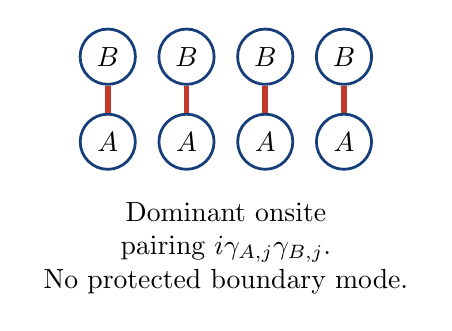
\begin{tikzpicture}[x=1.0cm,y=0.9cm]
  \foreach \j in {0,1,2,3} {
    \node[circle,draw=TitleBlue,line width=1pt,fill=white,minimum size=7mm] (A\j) at (\j,0) {$A$};
    \node[circle,draw=TitleBlue,line width=1pt,fill=white,minimum size=7mm] (B\j) at (\j,1.2) {$B$};
    \draw[WarnRed,line width=2pt] (A\j) -- (B\j);
  }
  \node[text width=4.8cm,align=center] at (1.5,-1.5) {Dominant onsite pairing \(i\gamma_{A,j}\gamma_{B,j}\).\\ No protected boundary mode.};
\end{tikzpicture}

\column{0.53\textwidth}
\centering
\textbf{Topological regime: \(\mu=0,\ t=\Delta\)}

\vspace{0.2cm}
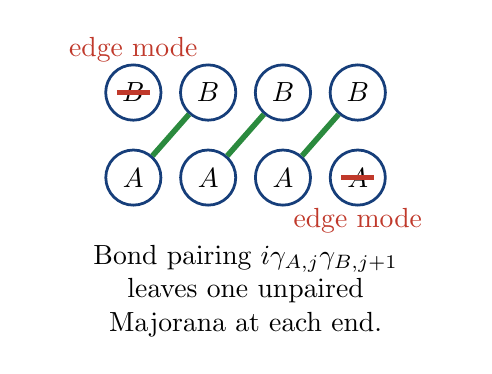
\begin{tikzpicture}[x=0.95cm,y=0.9cm]
  \foreach \j in {0,1,2,3} {
    \node[circle,draw=TitleBlue,line width=1pt,fill=white,minimum size=7mm] (A\j) at (\j,0) {$A$};
    \node[circle,draw=TitleBlue,line width=1pt,fill=white,minimum size=7mm] (B\j) at (\j,1.2) {$B$};
  }
  \foreach \j in {0,1,2} {
    \pgfmathtruncatemacro{\jp}{\j+1}
    \draw[TopGreen,line width=2pt] (A\j) -- (B\jp);
  }
  \draw[WarnRed,line width=2pt] (-0.22,1.2) -- (0.22,1.2);
  \draw[WarnRed,line width=2pt] (2.78,0) -- (3.22,0);
  \node[WarnRed,above] at (0,1.5) {edge mode};
  \node[WarnRed,below] at (3,-0.3) {edge mode};
  \node[text width=5.3cm,align=center] at (1.5,-1.6) {Bond pairing \(i\gamma_{A,j}\gamma_{B,j+1}\) leaves one unpaired Majorana at each end.};
\end{tikzpicture}
\end{columns}

\vspace{0.15cm}
\begin{align}
\mu=0,\ t=\Delta\quad \Longrightarrow \quad H_K = 2it\sum_{j=1}^{L-1}\gamma_{B,j+1}\gamma_{A,j}.
\end{align}
\end{frame}

\begin{frame}{4. From real space to BdG: Fourier transform and Nambu spinor}
\begin{columns}[T,totalwidth=\textwidth]
\column{0.54\textwidth}
Take periodic boundary conditions and define
\begin{align}
c_j=\frac{1}{\sqrt L}\sum_{k\in \mathrm{BZ}} c_k e^{ikj},\;
c_j^{\dagger}=\frac{1}{\sqrt L}\sum_{k\in \mathrm{BZ}} c_k^{\dagger} e^{-ikj}.
\end{align}

Then
\begin{align}
H_K = \sum_{k\in\mathrm{BZ}} \xi_k c_k^{\dagger}c_k
+i\Delta \sin k\left(c_k^{\dagger}c_{-k}^{\dagger}-c_{-k}c_k\right),
\end{align}
with
\begin{align}
\xi_k=-\mu-2t\cos k.
\end{align}

\column{0.42\textwidth}
Introduce the Nambu spinor
\begin{align}
\Psi_k^{\dagger}=\left(c_k^{\dagger},\ c_{-k}\right).
\end{align}
Then the Hamiltonian becomes a sum of \(2\times 2\) BdG blocks:
\begin{align}
H_K = \sum_{k>0} \Psi_k^{\dagger} h(k)\Psi_k 
\end{align}
with
\begin{align}
h(k)=
\begin{pmatrix}
\xi_k & 2i\Delta\sin k \\
-2i\Delta\sin k & -\xi_k
\end{pmatrix}.
\end{align}
\end{columns}
\end{frame}

\begin{frame}{5. BdG spectrum and the Dirac / two-band form}
\begin{columns}[T,totalwidth=\textwidth]
\column{0.55\textwidth}
The spectrum is
\begin{align}
E_k=\sqrt{(- \mu - 2 t \cos k)^2 + \left(2\Delta\sin k\right)^2}.
\end{align}
Hence the gap closes at
\begin{align}
\mu=\pm 2t.
\end{align}

Now rewrite the BdG matrix as a Dirac / two-band Hamiltonian
\begin{align}
h(k)=n_y(k)\sigma^y+n_z(k)\sigma^z,
\end{align}
with
\begin{align*}
n_y(k)=-2\Delta\sin k,\qquad n_z(k)=-\mu-2t\cos k.
\end{align*}

\column{0.42\textwidth}
\bluebox{This is the key geometric object. As \(k\) runs through the Brillouin zone, the vector
\begin{align}
\bm n(k)=\bigl(n_z(k),n_y(k)\bigr)
\end{align}
traces out a closed curve in the \((n_z,n_y)\) plane. The phase is determined by whether that curve winds around the origin.}
\end{columns}
\end{frame}

\begin{frame}{6. Winding number: does the closed curve wrap the origin?}
\small
\begin{columns}[T,totalwidth=\textwidth]
\column{0.48\textwidth}
Define
\begin{align}
\theta_k = \arg\!\bigl(n_z(k)+i n_y(k)\bigr).
\end{align}
Then the winding invariant is
\begin{align}
\nu = \frac{1}{2\pi}\int_{\mathrm{BZ}} \partial_k \theta_k\, dk.
\end{align}

\vspace{0.1cm}
Interpretation:
\begin{itemize}
  \item \(\nu=0\): the loop does \emph{not} enclose the origin
  \item \(|\nu|=1\): the loop encloses the origin once
  \item the only way to change \(\nu\) is for the loop to pass through the origin, i.e. for the bulk gap to close
\end{itemize}

\column{0.52\textwidth}
\centering
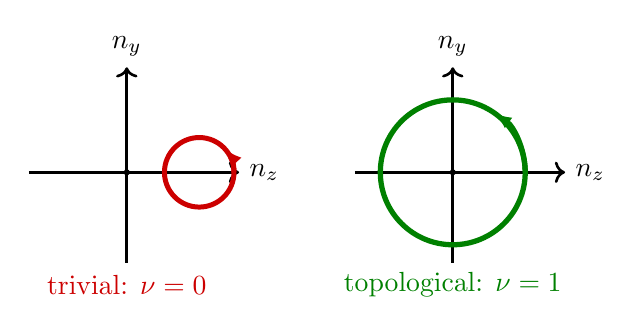
\begin{tikzpicture}[scale=0.92]
  % trivial panel
  \begin{scope}[shift={(-2.25,0)}]
    \draw[->,line width=0.95pt] (-1.35,0) -- (1.55,0) node[right] {$n_z$};
    \draw[->,line width=0.95pt] (0,-1.25) -- (0,1.45) node[above] {$n_y$};
    \fill[black] (0,0) circle (1.2pt);
    \draw[red!80!black,line width=1.8pt] (1,0) circle (0.48);
    \draw[red!80!black,line width=1.8pt,-{Latex[length=2.2mm]}] (1.48,0) arc[start angle=0,end angle=42,radius=0.48];
    \node[red!80!black] at (0,-1.55) {trivial: $\nu=0$};
  \end{scope}
  % topological panel
  \begin{scope}[shift={(2.25,0)}]
    \draw[->,line width=0.95pt] (-1.35,0) -- (1.55,0) node[right] {$n_z$};
    \draw[->,line width=0.95pt] (0,-1.25) -- (0,1.45) node[above] {$n_y$};
    \fill[black] (0,0) circle (1.2pt);
    \draw[green!50!black,line width=1.9pt] ( 0,0) circle (1.0);
    \draw[green!50!black,line width=1.9pt,-{Latex[length=2.2mm]}] (1.0,0.0) arc[start angle=0,end angle=55,radius=1.0];
    \node[green!50!black] at (0,-1.55) {topological: $\nu=1$};
  \end{scope}
\end{tikzpicture}
\end{columns}
\end{frame}

\begin{frame}{8. Infinite-chain spectrum}
\begin{columns}[T,totalwidth=\textwidth]
\column{0.44\textwidth}
Take an infinite translationally invariant chain with \(t=\Delta=1\). Then
\begin{align}
E_{\pm}(k)=\pm\sqrt{\bigl(-\mu-2\cos k\bigr)^2+4\sin^2 k}.
\end{align}
Representative cases:
\begin{itemize}
  \item \(\mu=-3\): trivial, gapped
  \item \(\mu=-2\): critical, gap closes at \(k=0\)
  \item \(\mu=-1\): topological, gapped
\end{itemize}

\vspace{0.08cm}

\column{0.56\textwidth}
\centering
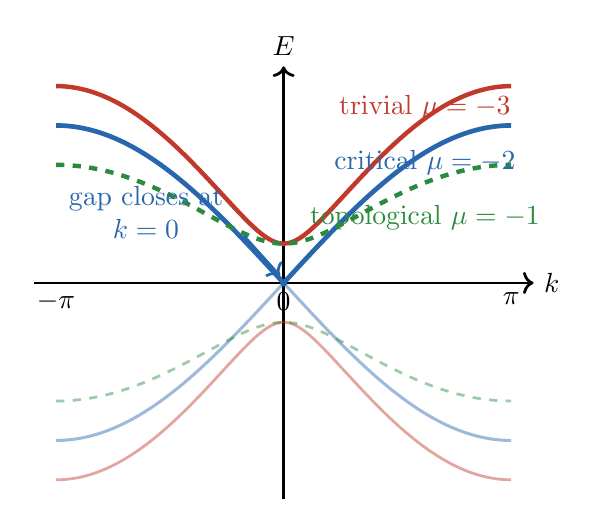
\begin{tikzpicture}[x=0.92cm,y=0.50cm]
  \draw[->,line width=1pt] (-3.45,0) -- (3.45,0) node[right] {$k$};
  \draw[->,line width=1pt] (0,-5.5) -- (0,5.5) node[above] {$E$};
  \node[below] at (-3.1416,0) {$-\pi$};
  \node[below] at (0,0) {$0$};
  \node[below] at (3.1416,0) {$\pi$};

  % trivial mu=-3
  \draw[WarnRed,line width=1.6pt,samples=200,smooth,domain=-3.1416:3.1416]
    plot (\x,{sqrt((3-2*cos(\x r))^2 + (2*sin(\x r))^2)});
  \draw[WarnRed,line width=1.0pt,opacity=0.45,samples=200,smooth,domain=-3.1416:3.1416]
    plot (\x,{-sqrt((3-2*cos(\x r))^2 + (2*sin(\x r))^2)});

  % critical mu=-2
  \draw[LineBlue,line width=1.7pt,samples=200,smooth,domain=-3.1416:3.1416]
    plot (\x,{sqrt((2-2*cos(\x r))^2 + (2*sin(\x r))^2)});
  \draw[LineBlue,line width=1.1pt,opacity=0.45,samples=200,smooth,domain=-3.1416:3.1416]
    plot (\x,{-sqrt((2-2*cos(\x r))^2 + (2*sin(\x r))^2)});

  % topo mu=-1
  \draw[TopGreen,line width=1.6pt,dashed,samples=200,smooth,domain=-3.1416:3.1416]
    plot (\x,{sqrt((1-2*cos(\x r))^2 + (2*sin(\x r))^2)});
  \draw[TopGreen,line width=1.0pt,opacity=0.45,dashed,samples=200,smooth,domain=-3.1416:3.1416]
    plot (\x,{-sqrt((1-2*cos(\x r))^2 + (2*sin(\x r))^2)});

  \fill[LineBlue] (0,0) circle (1.3pt);
  \node[WarnRed] at (1.95,4.45) {trivial \(\mu=-3\)};
  \node[LineBlue] at (1.95,3.05) {critical \(\mu=-2\)};
  \node[TopGreen] at (1.95,1.65) {topological \(\mu=-1\)};
  \draw[LineBlue,->,line width=1pt] (-0.55,1.2) -- (-0.05,0.18);
  \node[LineBlue,align=center] at (-1.9,1.8) {gap closes at\\$k=0$};
\end{tikzpicture}
\end{columns}
\end{frame}

\end{document}
